\subsubsection{Administrationsbereich}
\label{sec:Administrationsbereich}

Ein Oberflächenentwurf des Administrationsbereiches wird in folgender Abbildung dargestellt:

\begin{figure}[htb]
\centering
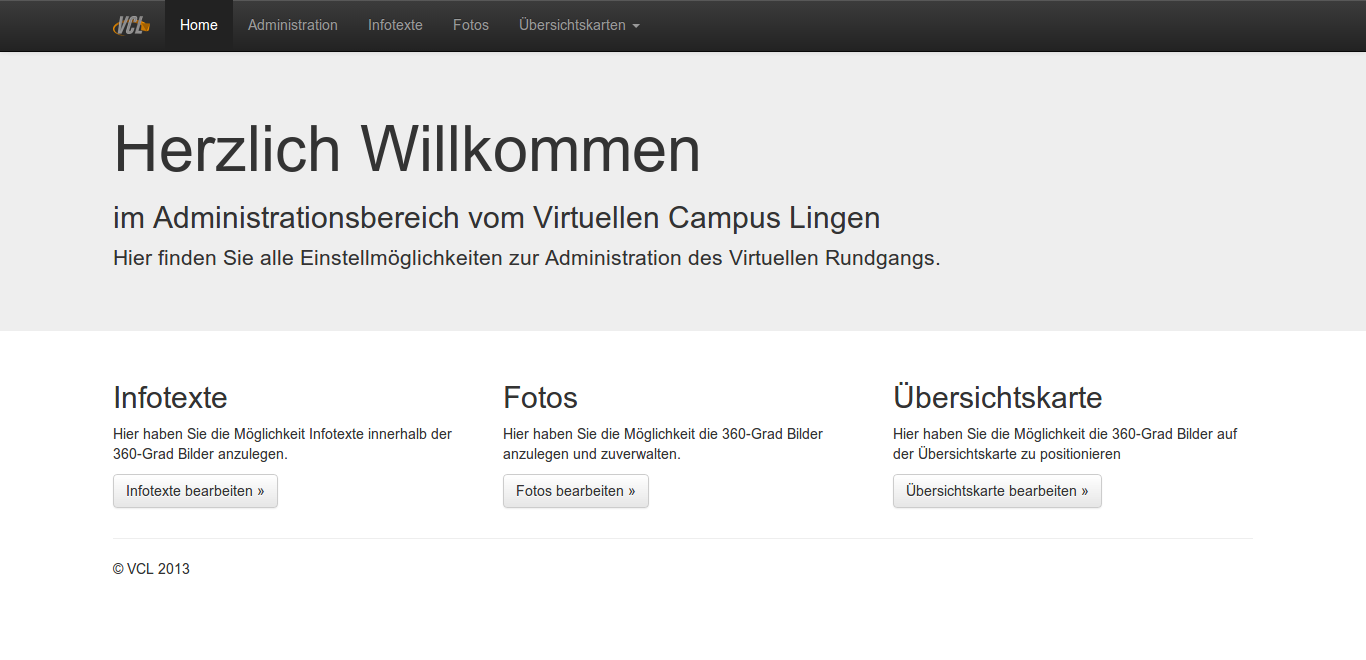
\includegraphics[width=1.0\textwidth]{MockupBackend.png}
\caption[Mockup Backend]{Oberflächenentwurf des
Administrationsbereiches\protect\footnotemark}
\label{fig:MockupBackend}
\end{figure}
\footnotetext{Quelle: Eigene Darstellung}

Der Administrationsbereich ist in vier Bereiche gegliedert:

\begin{itemize}
  \item Administrationsverwaltung
  \item Infotextverwaltung
  \item Fotoverwaltung
  \item Übersichtskarte
\end{itemize}

In der \textbf{Administrationsverwaltung} werden alle Informationen der Adminstratoren gepflegt. Zum Zeitpunkt der Erstellung des Mockups fällt darunter nur das Passwort und die Email-Adresse des Administrators. In diesem Menüpunkt können die Daten des angemeldeten Administrators, zum Beispiel Passwort und Email-Adresse, geändert werden. Die Erweiterung der Administratorinformationen ist jederzeit möglich.

In der \textbf{Infotextverwaltung} sollen Informationstexte zu einzelnen Panoramafotos hinterlegt und gepflegt werden. In diesem Bereich werden Informationstexte geschrieben und zu Panoramafotos zugeordnet. Ein Informationstext kann dabei auch mehreren Fotos zugeordnet werden. Dadurch können dem Benutzer alle Informationstexte angezeigt werden, die sich auf den Auschnitt des Campus beziehen, den er sich gerade ansieht. Alle Informationstexte, die bereits erstellt wurden, werden darüber hinaus tabellarisch angezeigt. Zu jedem angelegten Informationstext gibt es die Möglichkeit diesen zu verändern oder zu löschen.

In der \textbf{Fotoverwaltung} werden analog zu der Infotextverwaltung die erstellten Panoramafotos hinterlegt und gepflegt. Erstellte Panoramafotos können in diesem Menüpunkt mit Namen und Beschreibung hochgeladen werden. Analog zu den Infotexten werden auch die bereits hochgeladenen Fotos tabellarisch aufgelistet und mit der Möglichkeit zur Löschung bzw Änderung versehen.

% TODO: Anmerkung von Mkv -> er kann... unwissenschaftlich? Er-Form? Besser in 3 Person schreiben?

Die \textbf{Übersichtskarte} stellt den letzen und komplexesten Bereich des Administrationsbereiches dar. In der Übersichtskarte werden die hochgeladenen Panoramafotos auf einer Karte des Hochschulgebäudes platziert. Dazu wird dem angemeldeten Administrator eine Karte präsentiert und er kann durch auswählen eines Fotos und durch Klicken auf die Karte eine Position bestimmen an der das Foto gespeichert wird. Ein Foto kann dabei nur an einer Position auf der Übersichtskarte platziert werden. Der Administrator hat die Möglichkeit die Position jedes Fotos beliebig oft zu ändern. Darüber hinaus werden dem Administrator Steuerelemente (z.B in Form von Buttons) angezeigt mit denen er einen bestimmten Bereich des Hochschulcampus auswählen kann, zum Beispiel ein Gebäudetrakt oder ein Stockwerk in einem Gebäudetrakt. Neben der Möglichkeit ein Foto zu positionieren kann der Administrator im Menüpunkt der Übersichtskarte auch die Verbindung zwischen Fotos pflegen. Aus dem Oberflächenentwurf der Benutzeroberfläche im vorherigen Abschnitt ist ersichtlich, dass ein Benutzer von einem Panoramafoto zu einem anderen navigieren kann. Diese Navigation beruht auf Verbindungen zwischen den Panoramas. Diese Verbindungen werden in der Übersichtskarte geplegt. Die Steuerungselemente des Administrator zu Pflege dieser Verbindungen sind zum Zeitpunkt der Erstellung des Mockups noch nicht definiert, die Notwendigkeit dieser Funktion ist aber bedacht.